\section{Visual Aids User Study}\label{visual-aids-user-study}

goal: test whether users understand the mapping of 2d fold patterns to
3d, and test the degree to which plane coloring, edge patterning, and a
3d preview help users understand how a popup card will fold.

Since. \textgreater{}\textgreater{}TODO: cite other research on visual
aids for folding slash other 2d to 3d vis

\subsection{Method}\label{method}

Each subject received a set of five laser cut cards, and we recorded the
time it takes them to successfully fold the card.

For each card, each subject was randomly given one of of the following
five aids:

\begin{enumerate}
\def\labelenumi{\arabic{enumi})}
\itemsep1pt\parskip0pt\parsep0pt
\item
  A two-dimensional design, showing planes shaded by whether they will
  be horizontal or vertical when folded.
\item
  A two-dimensional design, with edges patterned based on whether they
  are ``hills'' or ``valleys'' --- whether they fold towards or away
  from the card.
\item
  A video showing a simulation of the card folding in three dimensions.
\item
  A still image of the card folded in dimension.
\item
  No visual aid.
\end{enumerate}

The order of aids and cards was shuffled, and then balanced to ensure an
equal distribution of orderings. Eg. each visual aid has an equal chance
of being the first aid presented to a user and

Finally, we asked subjects to rank the visual aids

The effect each type of aid has on folding time will help determine
which types of visualization to include in Foldlings

\subsection{Results and Discussion}\label{results-and-discussion}

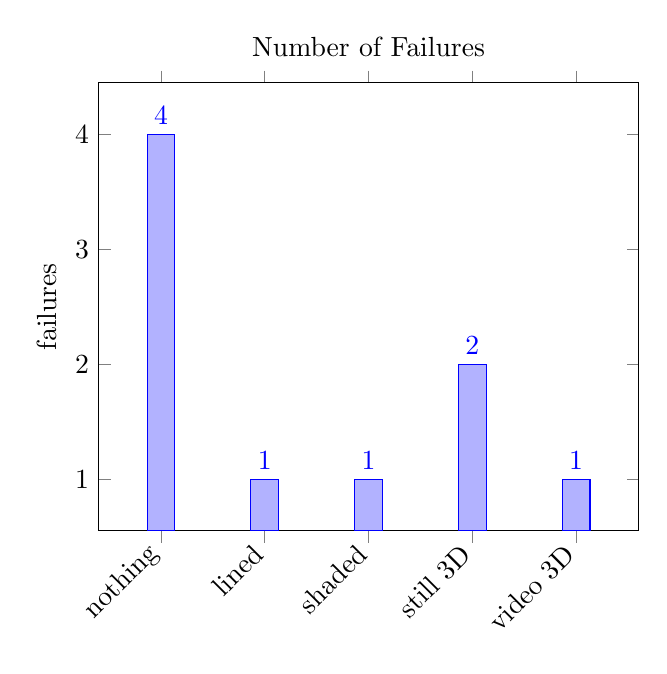
\begin{tikzpicture}
  \begin{axis}[
    title=Number of Failures,
    ybar,
    enlargelimits=0.15,
    legend style={at={(0.5,-0.2)},
      anchor=north,legend columns=-1},
    ylabel={failures},
    symbolic x coords={nothing,lined,shaded,still 3D,video 3D},
    xtick=data,
    nodes near coords, 
    nodes near coords align={vertical},
    x tick label style={rotate=45,anchor=east},
    ]
    \addplot coordinates {(nothing,4)(lined,1)(shaded,1)(still 3D,2)(video 3D,1)};
  \end{axis}
\end{tikzpicture}

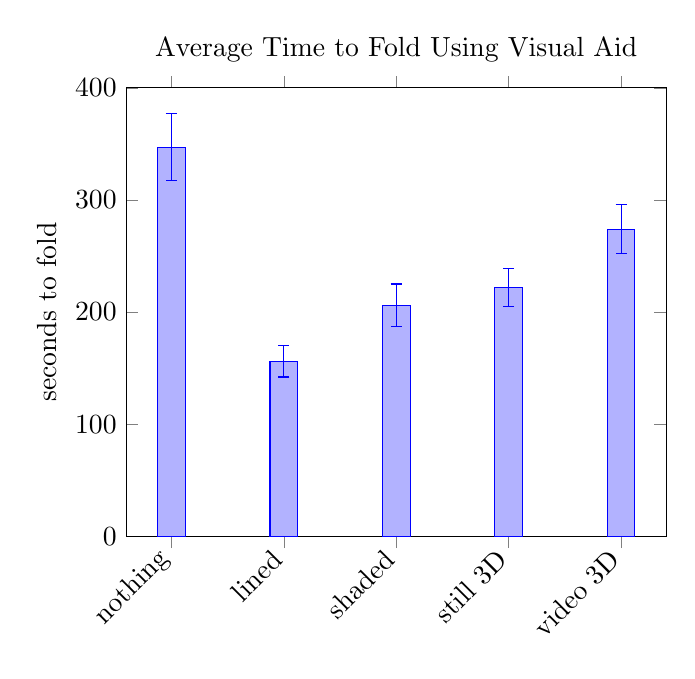
\begin{tikzpicture}
\begin{axis}[
  title=Average Time to Fold Using Visual Aid,
    ybar,
    ymin=0, ymax=400,
    legend style={at={(0.5,-0.2)},
     legend columns=-1},
    ylabel={seconds to fold},
    symbolic x coords={nothing,lined,shaded,still 3D,video 3D},
    xtick=data,
    x tick label style={rotate=45,anchor=east},
]
\addplot+[error bars/.cd,
y dir=both,y explicit]
coordinates {
    (nothing,347) +- (0.0, 30)
    (lined,156) +- (0.0, 14)
    (shaded,206) +- (0.0, 19)
    (still 3D,222) +- (0.0, 17)
    (video 3D,274) +- (0.0, 22)};
\end{axis}
\end{tikzpicture}

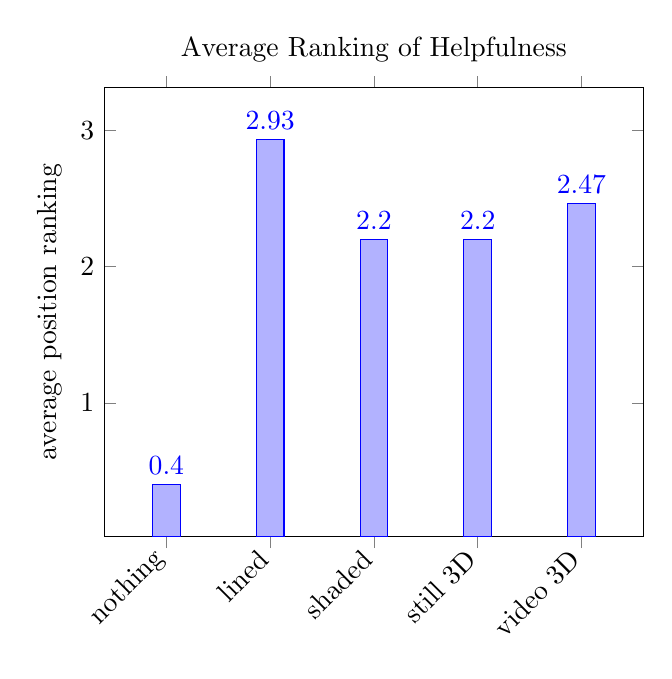
\begin{tikzpicture}
  \begin{axis}[
    title=Average Ranking of Helpfulness,
    ybar,
    enlargelimits=0.15,
    legend style={at={(0.5,-0.2)},
      anchor=north,legend columns=-1},
    ylabel={average position ranking},
    symbolic x coords={nothing,lined,shaded,still 3D,video 3D},
    xtick=data,
    nodes near coords, 
    nodes near coords align={vertical},
    x tick label style={rotate=45,anchor=east},
    ]
    \addplot coordinates {(nothing,0.4)(lined,2.933333333)(shaded,2.2)(still 3D,2.2)(video 3D,2.466666667)};
  \end{axis}
\end{tikzpicture}
